\documentclass{article}
\usepackage{arxiv}

\usepackage[utf8]{inputenc}
\usepackage[T1]{fontenc}
\usepackage{hyperref}
\usepackage{url}
\usepackage{booktabs}
\usepackage{amsfonts}
\usepackage{amsmath}
\usepackage{amssymb}
\usepackage{nicefrac}
\usepackage{microtype}
\usepackage{graphicx}
\usepackage{xcolor}
\usepackage{bm}
\usepackage[numbers]{natbib}
\usepackage{amsthm}
\usepackage{placeins}
\usepackage{tikz}
\usetikzlibrary{arrows.meta,positioning,calc,shapes.geometric,fit,backgrounds}

\newtheorem{definition}{Definition}

\title{Silent Zombies: Inference-Time Latent-Handoff Attacks that Drive
Unauthorized Actions in Tool-Using Multi-Agent Systems}

\author{%
  Virgile Thonnier\\
  KAIST, School of Computing\\
  IS-631 Kernel \& System Security\\
  \texttt{virgile.thonnier@kaist.ac.kr}\\
}

\renewcommand{\shorttitle}{Silent Zombies: Latent-Handoff Attacks on Tool-Using MAS}

\hypersetup{
  pdftitle={Silent Zombies: Latent-Handoff Attacks on Tool-Using Multi-Agent Systems},
  pdfauthor={Virgile Thonnier},
  pdfkeywords={multi-agent LLM security, latent communication, KV-cache attack,
               prompt injection, AgentDojo, TAMAS, LatentMAS, activation detection},
}

\begin{document}
\maketitle

\begin{abstract}
Multi-agent systems (MAS) built from large language models increasingly
communicate over a \emph{latent} channel: agents pass internal transformer
key--value (KV) attention caches or hidden states directly to one another
instead of natural-language text messages. This removes the assumption on which
current multi-agent monitors rely, namely that inter-agent messages are
human-readable text. We study the security consequences under a
single-compromise, inference-time, victim-unmodified threat model in which an
adversary overwrites only the latent handoff emitted by one compromised node
(the ``zombie'') without changing any other agent's weights, prompts, tools, or
emitted text. Across $24$ task-injection pairs spanning three AgentDojo
tool-use suites (\texttt{workspace}, \texttt{banking}, \texttt{slack}),
full-space projected gradient descent (PGD) on the latent KV handoff achieves a
$75.0\%$ attack success rate (ASR) against a $0.0\%$ clean baseline and a
$4.2\%$ text-channel baseline, while both a text/perplexity monitor and an
own-activation detector (AcMAS) record a $0.0\%$ catch rate. Across five
domains of Microsoft TAMAS ($20$ four-agent workflows), Silent Zombie latent PGD
reaches $100.0\%$ malicious tool execution at $0.0\%$ text catch, whereas an
active edge-level tensor reference monitor deployed at the inter-agent handoff
boundary catches $100.0\%$ of attacks and restores exact baseline security
($20.0\%$ ASR) and benign utility ($65.0\%$). On pure-latent multi-agent
reasoning (LatentMAS), latent communication cuts token generation by
$94.7\%$--$98.5\%$, yet full-space PGD hijacks $53.3\%$ of \texttt{GSM8K} and
$100.0\%$ of \texttt{ARC-Challenge} answers, whereas one-dimensional (1D)
activation steering fails ($0.0\%$). Controlled white-box comparisons show that
latent PGD achieves $62.5\%$ ASR versus $37.5\%$ for discrete token-level
Greedy Coordinate Gradient (GCG) attacks ($75.0\%$ caught by perplexity/text
filters), while inserting a single text conversation point---forcing an
intermediate agent to decode and re-encode a natural-language message---collapses
three-agent injection ASR from $62.5\%$ to $0.0\%$. Reusable $16$-slot
universal KV prefix patches (fixed virtual KV token blocks concatenated onto
any clean handoff) transfer zero-shot to $81.2\%$ of unseen tasks, and an
adaptive dual-evasion adversary can defeat unauthenticated statistical
monitors; however, enforcing keyed HMAC-SHA256 authentication on a POSIX
\texttt{/dev/shm} shared-memory tensor bus rejects $10/10$ bus-tampering
attempts (at a software hashing cost of $134$--$152$~MB/s), and query-only or
surrogate black-box attacks fail ($0.0\%$ ASR), establishing weight and
KV-schema confidentiality as a meaningful security perimeter.
\end{abstract}

\keywords{multi-agent LLM security \and latent communication \and KV-cache
attack \and prompt injection \and AgentDojo \and TAMAS \and activation detection}

% ===========================================================================
\section{Introduction}
\label{sec:intro}
Large language models are increasingly deployed not as single assistants but as
multi-agent systems (MAS), in which specialized agents---a planner, a critic, a
refiner, a tool executor, an aggregator---cooperate on complex tasks. In the
conventional design, agents exchange natural-language messages, so every
inter-agent edge is a readable string that an automated safety filter or human
auditor can inspect. A fast-growing line of work replaces this text bus with a
\emph{latent} channel in which agents pass hidden states or key--value (KV)
caches directly, avoiding the detokenize--retokenize round trip and cutting
inter-agent token generation by over an order of magnitude~\citep{latentmas,c2c}.
This architectural shift improves efficiency and expressiveness, but it also
eliminates the assumption that multi-agent monitors rely upon: that what one
agent transmits to another is text.

Initial studies of latent-channel vulnerabilities leave open the question that
governs deployed tool-using systems. Text-derived one-dimensional (1D) steering
adds a single fixed direction vector to degrade downstream QA
accuracy~\citep{outofsight}; norm-matched perturbations evade magnitude
detectors on single specialists~\citep{wlal}; and cache-reuse attacks corrupt
single-model answers~\citep{hijackkv}. None evaluate whether a single
compromised node can drive \emph{consequential, externally verified unauthorized
actions} across full tool-using benchmarks, how white-box latent attacks compare
against white-box discrete text attacks and intermediate text conversation
points, whether such attacks transfer zero-shot to unseen prompts or persist
under black-box constraints, and whether an operating-system (OS) edge monitor
over the transmitted KV tensor can close the gap.

We answer these questions with an end-to-end attack, defense, and OS-level
inter-process communication (IPC) evaluation spanning
AgentDojo~\citep{agentdojo}, Microsoft TAMAS~\citep{tamas}, and LatentMAS
reasoning benchmarks~\citep{latentmas,gsm8k,arc}. Throughout the paper, labels
\texttt{M3}--\texttt{M12} refer to our modular experiment suites (matching the
reproducible drivers \texttt{run\_m*.py} and archived JSON outputs in
\texttt{paper/results/}). Our evaluation establishes six core findings:
\begin{enumerate}
  \item \textbf{Latent handoffs amplify tool-hijacking while blinding text and
  activation monitors.} Across $24$ AgentDojo task-injection pairs, latent
  full-space PGD raises ASR from $0.0\%$ (clean) and $4.2\%$ (text baselines) to
  $75.0\%$, with $0.0\%$ detection by both text monitors and own-activation
  AcMAS (Activation-based Multi-Agent Security) probes~\citep{acmas}. On
  Microsoft TAMAS ($20$ workflows across $5$ domains), latent PGD achieves
  $100.0\%$ ASR vs.\ $95.0\%$ for text direct prompt injection (DPI), while
  dropping text catch rates from $100.0\%$ to $0.0\%$.
  \item \textbf{High-dimensional KV tensors strictly dominate 1D and discrete
  white-box attacks.} In a matched white-box comparison ($n=8$), full-space KV
  PGD achieves $62.5\%$ ASR (mean target negative log-likelihood, NLL, $0.029$)
  in $64.7$~s, whereas white-box discrete GCG~\citep{zou2023gcg} on text
  achieves $37.5\%$ ASR ($75.0\%$ caught) and 1D Out-of-Sight steering achieves
  $0.0\%$ ASR on tool calls and LatentMAS exact targets ($0.0\%$ on
  \texttt{GSM8K}/\texttt{ARC} vs.\ $53.3\%$/$100.0\%$ for full PGD).
  \item \textbf{Text conversation points impose a causal bottleneck, whereas
  pure-latent reasoning removes depth bounds.} In a three-agent pipeline,
  forcing agents to decode through even one text conversation boundary collapses
  ASR from $62.5\%$ to $0.0\%$ and yields $25.0\%$--$75.0\%$ text monitor catch.
  Conversely, removing intermediate text decodes in a differentiable pure-latent
  chain yields $100.0\%$ target control at every depth $2\dots 6$ ($n=3$) with
  non-vanishing initial gradient norms ($2.45$--$3.23$).
  \item \textbf{Universal latent prefix patches transfer zero-shot.} A reusable
  $16$-slot KV prefix patch (a fixed block of $16$ learned virtual KV token
  entries concatenated onto any clean handoff, trained once on $3$ tasks)
  transfers zero-shot ($0$ test-time optimization steps) to $16$ unseen tasks at
  $81.2\%$ ASR, $50.0\%$ on $3$-worker Star and $3$-hop pure-latent graphs, and
  $50.0\%$ under paraphrased prompts and reordered tool schemas ($n=6$).
  \item \textbf{Active edge monitoring restores baseline security, while adaptive
  dual evasion motivates cryptographic binding over OS shared memory.} Deployed
  at the inter-agent edge, \texttt{EdgeTensorReferenceMonitor} detects
  $100.0\%$ of TAMAS attacks (restoring exact $20.0\%$ clean ASR and $65.0\%$
  utility across all $5$ domains) and $100.0\%$ of LatentMAS hijacks. Under an
  adaptive dual-evasion adversary ($\lambda_{\text{edge}}=2500$), unauthenticated
  statistical checks can be evaded ($0.0\%$ flag rate at $100.0\%$ ASR), whereas
  HMAC-SHA256 authentication on our POSIX \texttt{/dev/shm} zero-copy tensor bus
  rejects $10/10$ bus-tampering attempts (revealing that software HMAC-SHA256 at
  $134$--$152$~MB/s dominates raw memory-mapped copy time).
  \item \textbf{Open weights define a sharp black-box security boundary.} Under
  strictly black-box threat regimes (zero victim gradients: full-space evolution
  strategies [ES], singular-value-decomposition [SVD] subspace natural evolution
  strategies [NES], decision-only string optimization, and unaligned or
  Cache-to-Cache [C2C] ridge-aligned~\citep{c2c} \texttt{1.5B}$\to$\texttt{3B}
  surrogates), unauthorized tool-call ASR drops to $0.0\%$ across all $6$
  regimes, showing that weight and KV-schema confidentiality remain an effective
  defense against external query-only adversaries.
\end{enumerate}

\paragraph{Scope and ethics.}
All evaluations run exclusively inside sandboxed mock environments (AgentDojo,
TAMAS synthetic workflows, and offline LatentMAS datasets). No real emails,
bank transfers, or harmful real-world payloads are executed.

% ===========================================================================
\section{Threat Model}
\label{sec:threat}

\begin{definition}[Latent multi-agent system and KV handoff]
A latent multi-agent system is a directed acyclic graph $G=(\mathcal V,\mathcal
E)$ whose nodes are LLM agents. Each agent is a frozen, aligned transformer
$f_\theta$ with $L$ layers wearing a fixed role (system prompt and JSON tool
schema) and executing a bounded \emph{Reason-and-Act (ReAct) loop}~\citep{yao2023react},
in which the agent iteratively emits structured tool calls
(\texttt{<tool\_call>...</tool\_call>}), runs them in a sandboxed environment,
appends tool observations to its context, and stops upon generating a final
answer. When an agent processes a prompt of $T$ tokens, each attention layer
$\ell \in \{0,\dots,L-1\}$ caches its projected key and value matrices
$K^{(\ell)}, V^{(\ell)} \in \mathbb{R}^{1 \times n_{\text{kv}} \times T \times d_h}$,
where $n_{\text{kv}}$ is the number of key--value attention heads and $d_h$ is
the per-head dimension. An edge $(u\!\to\!v)\in \mathcal E$ is a \emph{latent
handoff}: node $u$ transmits this KV cache tensor
$H_{u\to v}=\{(K^{(\ell)},V^{(\ell)})\}_{\ell=0}^{L-1}$ directly to $v$, which
prepends $H_{u\to v}$ to its own attention cache and attends over it directly
without decoding or reading natural-language text.
\end{definition}

\paragraph{Adversary.}
We consider both a primary \textbf{white-box single-compromise adversary} and a
spectrum of \textbf{black-box adversaries} (\texttt{M12}). In the white-box
setting, the adversary controls exactly one node $v_c$ (the \emph{zombie}) and
may overwrite the handoff $H_{c\to j}$ it emits on outgoing latent edges at
inference time, with full access to the graph topology, agent roles, and open
model weights $\theta$ so it can compute exact gradients $\nabla_\Delta\mathcal{L}$
via backpropagation. The adversary may not modify any other agent's weights,
prompt, tools, or decoding, may not alter user inputs or tool outputs, and adds
no trained module or fine-tuning to the victim. We stress that the attack is
\emph{not} optimization-free: the attacker runs inference-time PGD (per-query or
amortized offline into a reusable universal prefix patch) while leaving the
victim model completely unmodified. We explicitly avoid the misnomer
``training-free'', as continuous PGD optimization on the attacker side is
required even though the victim receives no weight updates. In our black-box
evaluation (\texttt{M12}), we remove access to victim weights and gradients
altogether, restricting the attacker to forward-pass log-probability queries
(\texttt{BB-0}, \texttt{BB-1}), decoded-text-only feedback (\texttt{BB-2}), or
an independent smaller surrogate model (\texttt{BB-3a}, \texttt{BB-3b}).

\paragraph{Defender.}
As illustrated in the topological threat diagram of Figure~\ref{fig:threat_topology},
the defender operates three concurrent inspection layers:
\begin{enumerate}
  \item A \textbf{text/perplexity (PPL) monitor} (\texttt{AgenticTextMonitor})
  inspecting every decoded inter-agent message and tool return for both lexical
  prompt-injection patterns (regular expressions matching override phrases or
  unauthorized tool names) and anomalous fluency---flagging high-perplexity
  adversarial token suffixes (mean per-token NLL above threshold or
  high-gibberish token ratios, characteristic of discrete GCG strings).
  \item An \textbf{activation-space detector (AcMAS)}~\citep{acmas}, which
  probes each text-generating agent's final-layer hidden state $h_j$ by
  measuring its cosine distance $1-\cos(h_j,\mu_j)$ to a calibrated
  role-specific benign centroid $\mu_j$ (flagging when distance exceeds
  $\tau=0.12$). Because a silent zombie node writes only KV tensors and emits
  no generated tokens, AcMAS has no generation-time probe point at $v_c$ itself
  and can only inspect downstream generating agents $v_j$.
  \item An \textbf{OS-level edge reference monitor} (\texttt{EdgeTensorReferenceMonitor})
  situated directly on the inter-agent POSIX \texttt{/dev/shm} shared-memory
  tensor bus (Linux's RAM-backed \texttt{tmpfs} filesystem enabling zero-copy
  \texttt{mmap} IPC between agent processes). Before the downstream executor
  ingests an incoming KV handoff, the monitor verifies a keyed
  \textbf{HMAC-SHA256} integrity tag (rejecting external tampering or bus
  spoofing) and evaluates three statistical anomaly signals over monitored
  layers $\mathcal{S}$: (i) \emph{position-pooled cosine distance}
  $1-\cos(\bar H, \mu_{\text{edge}})$, obtained by averaging keys and values
  across token positions into a length-invariant vector and comparing against a
  calibrated benign handoff centroid; (ii) \emph{per-layer Frobenius (L2) norm
  ratio} $\|H^{(\ell)}\|_F / \mu_{\text{norm}}^{(\ell)}$, detecting abnormal
  tensor energy inflation; and (iii) \emph{spectral concentration shift}
  $|\sigma_1(H^{(\ell)})/\|H^{(\ell)}\|_F - \mu_{\text{spec}}^{(\ell)}|$,
  measuring how strongly layer energy concentrates onto its top singular value
  $\sigma_1$ (specifically catching low-rank/1D steering directions even when
  global cosine shift is small). Upon rejection (\texttt{mode="gate"}), the
  runtime quarantines the poisoned KV cache and falls back to clean unperturbed
  context. Note that cryptographic HMAC authentication and statistical geometry
  gating are complementary: HMAC blocks external bus tampering ($100\%$
  rejection), whereas statistical gating catches an already-compromised zombie
  process that holds its own valid signing key.
\end{enumerate}

\begin{figure}[t]
\centering
\resizebox{\linewidth}{!}{%
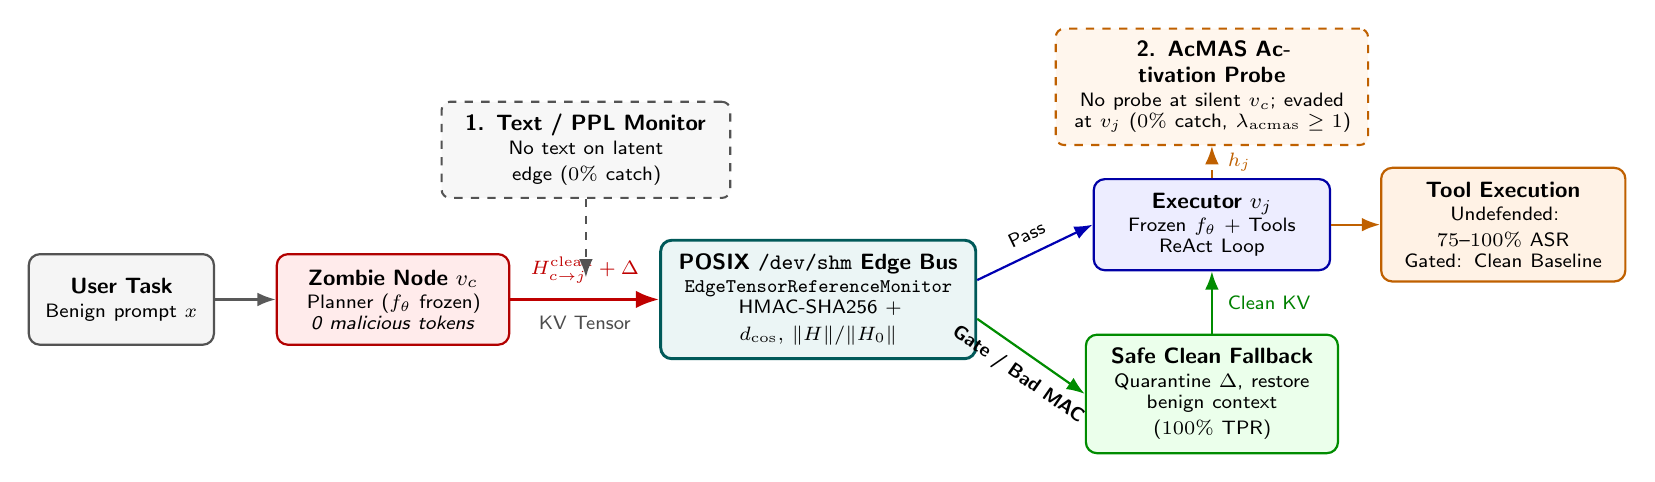
\begin{tikzpicture}[
  >=Latex,
  font=\sffamily\footnotesize,
  nodebox/.style={draw, rounded corners=4pt, align=center, minimum height=1.15cm, inner sep=5pt, line width=0.8pt},
  monbox/.style={draw, rounded corners=3pt, align=center, inner sep=4.5pt, line width=0.75pt}
]
  % Core pipeline nodes
  \node[nodebox, fill=gray!8, draw=gray!65!black, text width=2.0cm] (user) at (0, 0)
    {\textbf{User Task}\\[-1pt]{\scriptsize Benign prompt $x$}};

  \node[nodebox, fill=red!8, draw=red!70!black, text width=2.6cm] (zombie) at (3.45, 0)
    {\textbf{Zombie Node $v_c$}\\[-1pt]{\scriptsize Planner ($f_\theta$ frozen)}\\[-2pt]{\scriptsize \emph{0 malicious tokens}}};

  \node[nodebox, fill=teal!8, draw=teal!70!black, line width=1.05pt, text width=3.65cm] (bus) at (8.85, 0)
    {\textbf{POSIX \texttt{/dev/shm} Edge Bus}\\[-1pt]{\scriptsize \texttt{EdgeTensorReferenceMonitor}}\\[-2pt]{\scriptsize HMAC-SHA256 + $d_{\cos},\,\|H\|/\|H_0\|$}};

  \node[nodebox, fill=blue!7, draw=blue!65!black, text width=2.65cm] (exec) at (13.85, 0.95)
    {\textbf{Executor $v_j$}\\[-1pt]{\scriptsize Frozen $f_\theta$ + Tools}\\[-2pt]{\scriptsize ReAct Loop}};

  \node[nodebox, fill=green!8, draw=green!55!black, text width=2.85cm] (safe) at (13.85, -1.20)
    {\textbf{Safe Clean Fallback}\\[-1pt]{\scriptsize Quarantine $\Delta$, restore}\\[-2pt]{\scriptsize benign context ($100\%$ TPR)}};

  \node[nodebox, fill=orange!10, draw=orange!75!black, text width=2.75cm] (act) at (17.55, 0.95)
    {\textbf{Tool Execution}\\[-1pt]{\scriptsize Undefended: $75$--$100\%$ ASR}\\[-2pt]{\scriptsize Gated: Clean Baseline}};

  % Monitors (Blind / Bypassed)
  \node[monbox, dashed, fill=gray!6, draw=gray!65!black, text width=3.35cm] (txtmon) at (5.90, 1.90)
    {\textbf{1. Text / PPL Monitor}\\[-1pt]{\scriptsize No text on latent edge ($0\%$ catch)}};

  \node[monbox, dashed, fill=orange!7, draw=orange!75!black, text width=3.65cm] (acmas) at (13.85, 2.70)
    {\textbf{2. AcMAS Activation Probe}\\[-1pt]{\scriptsize No probe at silent $v_c$; evaded}\\[-2pt]{\scriptsize at $v_j$ ($0\%$ catch, $\lambda_{\mathrm{acmas}}\ge 1$)}};

  % Edges
  \draw[->, thick, draw=gray!70!black] (user.east) -- (zombie.west);
  \draw[->, very thick, draw=red!75!black] (zombie.east) --
    node[above=2pt, font=\sffamily\scriptsize\bfseries, text=red!75!black] {$H^{\mathrm{clean}}_{c\to j} + \Delta$}
    node[below=2pt, font=\sffamily\scriptsize, text=gray!60!black] {KV Tensor} (bus.west);

  \draw[->, dashed, thick, draw=gray!65!black] (txtmon.south) -- (5.90, 0.28);
  \draw[->, dashed, thick, draw=orange!75!black] (exec.north) --
    node[right=2pt, font=\sffamily\scriptsize, text=orange!75!black] {$h_j$} (acmas.south);

  \draw[->, thick, draw=blue!70!black] ([yshift=7pt]bus.east) --
    node[above=1pt, sloped, font=\sffamily\scriptsize] {Pass} (exec.west);

  \draw[->, thick, draw=green!55!black] ([yshift=-7pt]bus.east) --
    node[below=1pt, sloped, font=\sffamily\scriptsize\bfseries] {Gate / Bad MAC} (safe.west);

  \draw[->, thick, draw=green!55!black] (safe.north) --
    node[right=2pt, font=\sffamily\scriptsize, text=green!50!black] {Clean KV} (exec.south);

  \draw[->, thick, draw=orange!75!black] (exec.east) -- (act.west);
\end{tikzpicture}}
\caption{Topological threat model and defense interposition in a latent multi-agent
system $G=(\mathcal{V},\mathcal{E})$. Compromised node $v_c$ emits no malicious text,
blinding surface text monitors (1) and offering no generation probe to own-activation
detectors (2), while \texttt{EdgeTensorReferenceMonitor} (3) interposes directly on
the POSIX \texttt{/dev/shm} KV handoff edge $(c\!\to\!j)$.}
\label{fig:threat_topology}
\end{figure}

% ===========================================================================
\section{Testbed and Experimental Setup}
\label{sec:setup}

\paragraph{Hardware and OS environment.}
The complete validation suite (\texttt{M3}, \texttt{M4d}, \texttt{M6}--\texttt{M12})
executes inside a Linux environment running Ubuntu~24.04.4~LTS with Linux kernel
\texttt{6.6.159+} (\texttt{x86\_64}), equipped with an NVIDIA Tesla~T4 GPU
($14.56$~GB VRAM, compute capability \texttt{sm\_75}) and $50$~GiB system RAM,
using Python~3.13.16, PyTorch~2.14.1+cu130, CUDA~13.0, \texttt{transformers}~4.53.3,
\texttt{bitsandbytes}~0.50.2, and \texttt{agentdojo}~0.1.35. Because \texttt{sm\_75}
hardware lacks native Tensor Core \texttt{bfloat16} acceleration (which falls
back to slow software emulation), all primary T4 runs execute in hardware
\texttt{float16} compute over 4-bit \emph{NormalFloat} (NF4) double-quantized
weights~\citep{dettmers2023qlora} (QLoRA-style weight compression allowing a
3B-parameter model plus PGD backpropagation to fit inside $15$~GB VRAM) using
PyTorch's fused Scaled Dot-Product Attention (SDPA) kernel. Early topology and
stealth baselines (\texttt{M4}, \texttt{M4b}, \texttt{M4c}, \texttt{M5}) ran on
an $8$~GB NVIDIA RTX~2080~SUPER with \texttt{bfloat16} compute.

\paragraph{Backbone and latent channel.}
All victim agents share \texttt{Qwen2.5-3B-Instruct}~\citep{qwen25} ($L=36$
layers, hidden width $2048$, grouped-query attention [GQA] in which query heads
share $n_{\text{kv}}=2$ KV heads of dimension $d_h=128$ per layer). The planner
builds a KV cache over the benign user context; that tensor is prepended to
downstream agents' attention caches across all layers without textual
serialization.

\paragraph{OS-level IPC bus and reference monitor.}
To ground latent MAS handoffs in systems reality, we implement
\texttt{SharedMemoryTensorBus} backed by POSIX \texttt{/dev/shm} memory-mapped
buffers. Each handoff packs contiguous layer buffers alongside a fixed binary
header carrying shape, sequence nonce, and dtype metadata plus a $32$-byte
HMAC-SHA256 tag computed over header and payload bytes. On receipt,
\texttt{EdgeTensorReferenceMonitor} verifies the MAC and computes the three
statistical signals defined in Section~\ref{sec:threat} (cosine distance, norm
ratio, and spectral concentration shift), blocking or quarantining anomalous
edges before downstream attention.

\paragraph{Benchmarks and evaluation metrics.}
We evaluate across four complementary testbeds:
(i) \textbf{AgentDojo}~\citep{agentdojo} ($24$ pairs across \texttt{workspace}
email/calendar/files, \texttt{banking} transfers, and \texttt{slack} messaging),
where each pair combines a benign user request with an attacker injection goal
inside a sandboxed mock environment;
(ii) \textbf{Microsoft TAMAS} (\emph{Threats and Attacks in Multi-Agent
Systems})~\citep{tamas} ($20$ four-agent workflows spanning \texttt{finance},
\texttt{healthcare}, \texttt{legal}, \texttt{education}, and \texttt{news}),
comparing clean runs, text Direct Prompt Injection (DPI---explicit malicious
instructions appended to the user query), and latent attacks;
(iii) \textbf{LatentMAS} four-agent collaborative reasoning
(\texttt{Planner}$\to$\texttt{Critic}$\to$\texttt{Refiner}$\to$\texttt{Judger})~\citep{latentmas}
on \textbf{GSM8K}~\citep{gsm8k} (grade-school arithmetic word problems) and
\textbf{ARC-Challenge}~\citep{arc} (multiple-choice science questions), $n=15$
per dataset, measuring both token savings and exact-target wrong-answer
hijacking; and
(iv) \textbf{synthetic multi-topology graphs} (chain, star, tree, reconvergent
DAG, and pure-latent chains of depth $2$--$6$), where \emph{reach}
(forced-marker survival) measures whether a perturbation injected only at the
root planner causes a downstream agent $k$ hops away to emit a benign sentinel
word (\texttt{"BANANA"}), isolating multi-hop propagation from tool schemas.

Across these testbeds we report five core metrics: \textbf{Attack Success Rate
(ASR)} is the fraction of trials in which the unauthorized action or wrong
target answer actually executes and passes programmatic post-execution
verification (note that AgentDojo names its injection-success predicate
\texttt{security}: \texttt{security=true} means the \emph{attack succeeded} and
breached the environment, whereas \texttt{security=false} means the environment
remained safe); \textbf{Benign Utility} is the fraction of trials completing
the user's original benign task; \textbf{Target Negative Log-Likelihood (NLL)}
is $-\sum_{t=1}^{m}\log p_\theta(s_t\mid\dots)$ summed over the $m$ tokens of
the target unauthorized tool call ($\text{NLL}\approx 0$ indicates near-$100\%$
probability of emitting the exact unauthorized call, while $\text{NLL}\sim 100$
indicates near-zero probability); and detector \textbf{True Positive Rate (TPR)}
and \textbf{False Positive Rate (FPR)} are the fractions of attacked and clean
handoffs flagged, respectively. On TAMAS, the small $3$B backbone already
invokes sensitive target tools unprompted on $20.0\%$ of clean workflows
(concentrated in \texttt{news} and \texttt{healthcare}), establishing the clean
baseline floor that an ideal defense restores.

% ===========================================================================
\section{Method}
\label{sec:method}

\paragraph{Full-space KV PGD.}
On compromised edge $(c\!\to\!j)$, the adversary replaces the clean KV handoff
$H^{\mathrm{clean}}_{c\to j}$ (of prompt length $T$) with
$H^{\mathrm{clean}}_{c\to j}+\Delta$, where
$\Delta=\{\Delta_K^{(\ell)},\Delta_V^{(\ell)}\}_{\ell\in\mathcal S}$ optimizes
\emph{all coordinates} across both key and value tensors (\texttt{K+V}
``carriers''), all KV heads, and all $T$ positions within a chosen subset of
transformer layers $\mathcal S$ (e.g., $\mathcal S=\{20,24,28,32\}$). Treating
downstream prompt tokens $x_j$ and frozen weights $\theta$ as differentiable
context, the attacker minimizes \emph{teacher-forced} target tool-call negative
log-likelihood---scoring every target token $s_t$ conditioned on the exact
preceding target tokens $s_{<t}$ in a single differentiable forward pass:
\begin{equation}
\label{eq:obj}
\mathcal L(\Delta) \;=\; -\sum_{t=1}^{m}
\log p_\theta\!\big(s_t \mid s_{<t},\, H^{\mathrm{clean}}_{c\to j}+\Delta,\, x_j\big),
\end{equation}
using Adam ($\text{lr}=0.02$) followed after each step by a per-layer L2
norm-ball projection capped by multiplicative norm ratio $\rho \in \{4,8,16\}$:
\begin{equation}
\label{eq:proj}
\big\lVert H^{\mathrm{clean},(\ell)}+\Delta^{(\ell)}\big\rVert_2
\;\le\; \rho\,\big\lVert H^{\mathrm{clean},(\ell)}\big\rVert_2.
\end{equation}

\paragraph{White-box baselines and text conversation points (\texttt{M9}).}
To isolate why high-dimensional continuous KV caches outperform discrete or
low-rank attacks, \texttt{M9} Part~A compares full-space KV PGD against:
(a) white-box discrete \textbf{GCG} (Greedy Coordinate Gradient)~\citep{zou2023gcg},
which optimizes a $12$-token adversarial text suffix by swapping discrete tokens
using embedding gradients, either transmitted as plain text
(\texttt{wb\_gcg\_text\_on\_text\_comm}) or inserted into the zombie prompt and
passed through its KV cache (\texttt{wb\_gcg\_text\_on\_latent\_comm}); and
(b) \textbf{1D Out-of-Sight (OoS)} steering~\citep{outofsight}, which computes
a single fixed rank-$1$ displacement direction between malicious and benign
prompts and adds a scaled copy ($\rho=8$) to the KV cache.
In \texttt{M9} Part~B, we test the causal effect of \textbf{text conversation
points}---inter-agent boundaries where an agent must decode its internal state
into a natural-language message that the next agent re-encodes---in a
three-agent pipeline (\texttt{Planner}$\to$\texttt{Coordinator}$\to$\texttt{Executor}):
\texttt{0\_conv\_pure\_latent} passes KV caches on both edges ($0$ text
boundaries, enabling end-to-end 2-hop PGD); \texttt{1\_conv\_late\_unadapted}
inserts a text decode/re-encode step between Coordinator and Executor without
adapting the 1-hop PGD perturbation; \texttt{1\_conv\_late\_relay\_adapted}
explicitly optimizes the 1-hop PGD perturbation to make the Coordinator
verbalize the malicious instruction into its text message;
\texttt{1\_conv\_early\_wb\_text} places the text boundary first (using white-box
GCG) followed by a latent handoff; and \texttt{2\_conv\_all\_text} uses text on
both edges.

\paragraph{Zero-shot universal KV payloads (\texttt{M10}).}
Standard per-query KV PGD cannot transfer directly to unseen tasks because its
perturbation $\Delta$ has the exact sequence length $T$ of one specific prompt,
whereas an unseen prompt has a different length $T'\neq T$. To achieve
\emph{zero-shot} transfer ($0$ optimization steps at test time), we train two
length-agnostic payloads offline over three source tasks
(\texttt{user\_task\_0..2}) on layers $\mathcal{S}=\{20,24,28,32\}$ ($\rho=8$):
\begin{enumerate}
  \item \textbf{1-Slot Broadcast Delta:} a single learned key/value vector per
  attacked layer, $\Delta K_{\mathrm{bcast}}^{(\ell)}, \Delta V_{\mathrm{bcast}}^{(\ell)}
  \in \mathbb{R}^{1 \times n_{\text{kv}} \times 1 \times d_h}$, broadcast
  (added) identically across every token position $1\dots T'$ of any unseen
  clean handoff:
  $K_{\mathrm{out}}^{(\ell)} = K_{\mathrm{clean}}^{(\ell)} + \Delta K_{\mathrm{bcast}}^{(\ell)}$
  (and analogously for $V$).
  \item \textbf{16-Slot Universal KV Prefix Patch:} a fixed block of $P=16$
  learned \emph{virtual KV token slots} of shape
  $(1, n_{\text{kv}}, 16, d_h)$ per layer---analogous to prefix-tuning KV
  states. We initialize a neutral $16$-token base cache
  $(K_{\mathrm{base}}^{(\ell)}, V_{\mathrm{base}}^{(\ell)})$ across all $36$
  layers from a benign filler string, then jointly optimize trainable offsets
  $(\Delta K_{\mathrm{patch}}^{(\ell)}, \Delta V_{\mathrm{patch}}^{(\ell)})$ on
  $\ell \in \mathcal{S}$ over the $3$ training tasks. At test time on any
  unseen prompt of arbitrary length $T'$, the zombie leaves the clean tokens
  untouched and \emph{concatenates} the $16$ virtual slots along the sequence
  dimension onto the end of the clean handoff:
  \begin{equation}
  \label{eq:kvpatch}
  K_{\mathrm{out}}^{(\ell)} = \big[K_{\mathrm{clean}}^{(\ell)} \;\big\|\; K_{\mathrm{base}}^{(\ell)} + \Delta K_{\mathrm{patch}}^{(\ell)}\big],
  \qquad
  V_{\mathrm{out}}^{(\ell)} = \big[V_{\mathrm{clean}}^{(\ell)} \;\big\|\; V_{\mathrm{base}}^{(\ell)} + \Delta V_{\mathrm{patch}}^{(\ell)}\big],
  \end{equation}
  producing a $(T'+16)$-slot KV prefix consumed directly by the downstream
  executor with zero test-time gradient steps.
\end{enumerate}
We evaluate both payloads zero-shot across three axes: \textbf{Cross-Task}
($16$ unseen prompt/injection pairs), \textbf{Cross-Topology} ($3$-worker Star
fan-out, $3$-hop pure-latent chain, and a \emph{reconvergent DAG} merging either
one patched branch with one clean branch, $[H_{\text{patch}}\|H_{\text{clean}}]$,
or naively duplicating the same patch on both branches,
$[H_{\text{patch}}\|H_{\text{patch}}]$), and \textbf{Cross-Schema} (a
paraphrased executor system prompt combined with reversed tool-definition order).

\paragraph{Adaptive dual evasion (\texttt{M5}, \texttt{M8}).}
To test whether an attacker who knows our statistical detectors can evade them
simultaneously, we augment Eq.~\eqref{eq:obj} with differentiable penalties
pulling both the downstream agent's hidden state $h_j(\Delta)$ toward its clean
AcMAS centroid $\mu_j$ and the position-pooled handoff $\bar H(\Delta)$ toward
the Edge Monitor's benign centroid $\bar H_{\mathrm{ref}}$ (plus a relative L2
norm term with $\alpha=0.1$):
\begin{equation}
\label{eq:dualstealth}
\min_{\Delta}\; \mathcal L(\Delta)
\;+\; \lambda_{\mathrm{acmas}}\big(1-\cos(h_j(\Delta),\mu_j)\big)
\;+\; \lambda_{\mathrm{edge}}\Big(\big(1-\cos(\bar H(\Delta),\bar H_{\mathrm{ref}})\big) + \alpha\big(\|\Delta\|/\|H^{\mathrm{clean}}\|\big)^2\Big),
\end{equation}
conducting a \emph{Pareto sweep} over $\lambda_{\mathrm{acmas}}\in[0,50]$ and
$\lambda_{\mathrm{edge}}\in[0,2500]$ to map the trade-off between attack
success and detector evasion.

\paragraph{Black-box threat spectrum (\texttt{M12}).}
To probe whether external adversaries can mount silent zombie attacks without
victim weights or gradients (\texttt{torch.no\_grad}), we test six regimes:
\textbf{\texttt{BB-0} (Full-Space ES)}: gradient-free Evolution Strategies
perturbing the full KV tensor with isotropic Gaussian noise using only target
log-probability queries ($60$ queries);
\textbf{\texttt{BB-1} (SVD Subspace NES)}: Natural Evolution Strategies
restricting search to a low-rank ($r=16$) orthonormal basis built via Singular
Value Decomposition (SVD) of benign-vs.-malicious KV differences, scaling
perturbation noise $\sigma_\ell=0.25\|K_\ell\|$ and step size
$\text{lr}_\ell=0.45\|K_\ell\|$ across antithetic ($\pm$) pairs ($241$
queries);
\textbf{\texttt{BB-2} (Decision-Only Search)}: hard-label search observing
\emph{only the final decoded text} (zero logits) over $25$ rollouts using a
discrete string reward ($+1$ for valid \texttt{<tool\_call>} syntax, $+2$ for
matching target tool name, up to $+3$ for matching target arguments); and
\textbf{\texttt{BB-3a/b} (Cross-Model Surrogate \& C2C Bridge)}: optimizing a
$16$-slot KV patch white-box on a smaller surrogate
(\texttt{Qwen2.5-1.5B-Instruct}) and transferring it to the $3$B victim either
directly unaligned (\texttt{BB-3a}) or mapped through a closed-form linear
ridge-regression Cache-to-Cache (C2C) projection matrix fitted on aligned
benign prompts~\citep{c2c} (\texttt{BB-3b}, evaluated both at $0$ victim
queries and after query-based scale refinement).

% ===========================================================================
\section{Results}
\label{sec:results}

\subsection{Single-Edge Action Forcing on AgentDojo (\texttt{M3})}
\label{sec:results-m3}
On AgentDojo \texttt{workspace} (\texttt{user\_task\_0} + \texttt{injection\_task\_0}),
the clean executor benignly queries the calendar and leaves the sandbox safe
(AgentDojo's injection-success flag \texttt{security=false}). Table~\ref{tab:m3}
shows that all four PGD layer/budget configurations---targeting either $4$ late
layers (\texttt{late4\_n8}), $4$ evenly spaced layers (\texttt{spread4\_n8},
\texttt{spread4\_n16}), or $6$ deep layers (\texttt{deep6\_n16}) under norm cap
$\rho\in\{8,16\}$---drive exact target \texttt{send\_email} negative
log-likelihood from $118.37$ ($117.89$ for 6 layers) below $10^{-2}$ within
$\sim 40$ steps (Figure~\ref{fig:m3}), achieving $100\%$ forced greedy decoding
match and verified unauthorized email execution (\texttt{security=true}).

\begin{table}[t]
\centering
\caption{M3 perturbation-budget and layer-placement sweep on AgentDojo
\texttt{workspace} (\texttt{user\_task\_0} + \texttt{injection\_task\_0},
\texttt{Qwen2.5-3B-Instruct} 4-bit NF4). Clean baseline leaves the sandbox safe
(\texttt{security=false}); \texttt{security=true} denotes verified unauthorized
tool execution (attack success).}
\label{tab:m3}
\begin{tabular}{llccccc}
\toprule
Configuration & Layers $\mathcal S$ & Carriers & $\rho$ & Final NLL & Forced Decode & Security \\
\midrule
\texttt{late4\_n8}   & $\{30,31,32,33\}$       & K+V & $8$  & $0.009$ & hit & true \\
\texttt{spread4\_n8} & $\{20,24,28,32\}$       & K+V & $8$  & $0.005$ & hit & true \\
\texttt{spread4\_n16}& $\{20,24,28,32\}$       & K+V & $16$ & $0.005$ & hit & true \\
\texttt{deep6\_n16}  & $\{12,16,20,24,28,32\}$ & K+V & $16$ & $0.005$ & hit & true \\
\bottomrule
\end{tabular}
\end{table}

\begin{figure}[t]
\centering
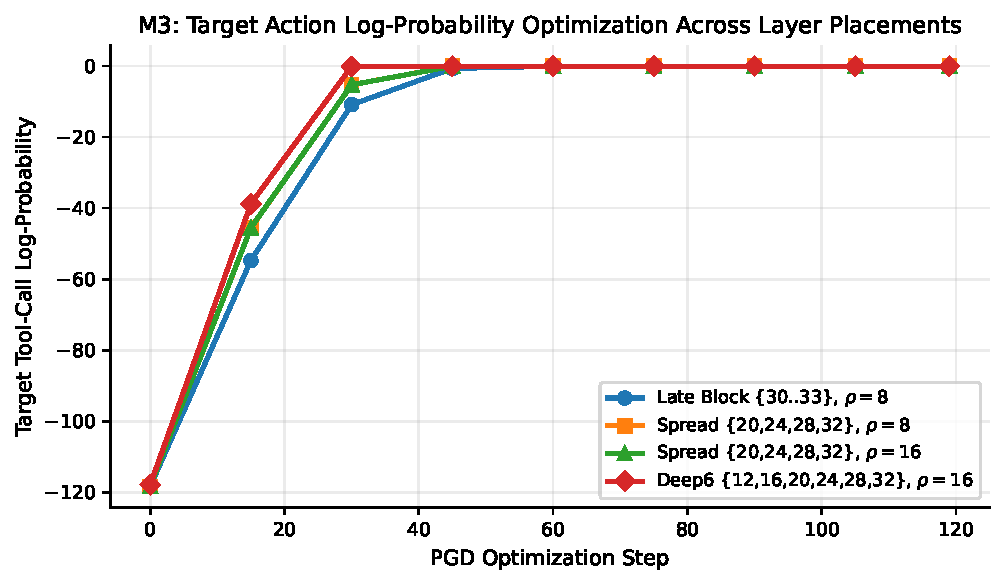
\includegraphics[width=0.72\linewidth]{figures/fig2_m3_nll_convergence.pdf}
\caption{M3 target tool-call log-probability trajectory across $120$ PGD steps
for all four layer placements and budgets.}
\label{fig:m3}
\end{figure}

\subsection{White-Box Expressivity Matrix and Text Conversation Points (\texttt{M9})}
\label{sec:results-m9}
Table~\ref{tab:m9} and Figure~\ref{fig:m9} resolve two crucial methodological
questions ($n=8$ matched AgentDojo task-injection pairs):
\begin{enumerate}
  \item \textbf{Channel \& degrees-of-freedom (DOF) advantage:} High-dimensional continuous KV PGD
  achieves $62.5\%$ ASR (mean target NLL $0.029$) in $64.74$~s while completely
  evading text/perplexity ($0.0\%$) and AcMAS ($0.0\%$) monitors. White-box GCG
  in text space achieves only $37.5\%$ ASR despite taking nearly twice as long
  ($116.39$~s) and is flagged at $75.0\%$ by perplexity/text checks; applying GCG
  into a latent handoff yields $0.0\%$ ASR (NLL $72.829$), and 1D Out-of-Sight
  steering fails completely ($0.0\%$ ASR, NLL $699.344$, $100.0\%$ flagged by
  both AcMAS and Edge detectors).
  \item \textbf{Causal effect of conversation boundaries:} In a three-agent
  pipeline (\texttt{Planner}$\to$\texttt{Coordinator}$\to$\texttt{Executor}), zero
  text conversation points (\texttt{0\_conv\_pure\_latent}) yields $62.5\%$ ASR
  and $0.0\%$ text detection. Inserting even a \emph{single} text decode/re-encode
  conversation boundary collapses end-to-end ASR to $0.0\%$ across all four
  variants (late unadapted, late relay-adapted, early GCG, or two-point full
  text) while restoring $25.0\%$--$75.0\%$ text monitor catch rates.
\end{enumerate}

\begin{table}[t]
\centering
\caption{M9 Part A (white-box 2$\times$2 expressivity matrix) and Part B
(three-agent text conversation-point ablation), $n=8$ pairs per row.}
\label{tab:m9}
\resizebox{\linewidth}{!}{%
\begin{tabular}{lccccc}
\toprule
Regime & ASR (\%) & Utility (\%) & Mean NLL & Text/PPL Catch & AcMAS / Edge Catch \\
\midrule
\multicolumn{6}{l}{\emph{Part A: White-Box Channel \& Subspace Expressivity ($n=8$)}} \\
\texttt{clean} & $0.0$ & $0.0$ & $95.811$ & $0.0\%$ & $0.0\%$ / $0.0\%$ \\
\texttt{wb\_gcg\_text\_on\_text\_comm} & $37.5$ & $25.0$ & $5.492$ & $75.0\%$ & $0.0\%$ / $0.0\%$ \\
\texttt{wb\_gcg\_text\_on\_latent\_comm} & $0.0$ & $0.0$ & $72.829$ & $0.0\%$ & $0.0\%$ / $100.0\%$ \\
\texttt{outofsight\_1d\_on\_latent\_comm} & $0.0$ & $0.0$ & $699.344$ & $0.0\%$ & $100.0\%$ / $100.0\%$ \\
\texttt{wb\_fullspace\_pgd\_on\_latent\_comm} & $\mathbf{62.5}$ & $0.0$ & $\mathbf{0.029}$ & $0.0\%$ & $0.0\%$ / $50.0\%$ \\
\midrule
\multicolumn{6}{l}{\emph{Part B: Causal Text Conversation Points in 3-Agent Pipeline ($n=8$)}} \\
\texttt{0\_conv\_pure\_latent} (0 text pts) & $\mathbf{62.5}$ & $0.0$ & --- & $0.0\%$ & --- \\
\texttt{1\_conv\_late\_unadapted} (1 pt) & $0.0$ & $12.5$ & --- & $25.0\%$ & --- \\
\texttt{1\_conv\_late\_relay\_adapted} (1 pt) & $0.0$ & $12.5$ & --- & $75.0\%$ & --- \\
\texttt{1\_conv\_early\_wb\_text} (1 pt) & $0.0$ & $0.0$ & --- & $75.0\%$ & --- \\
\texttt{2\_conv\_all\_text} (2 pts) & $0.0$ & $12.5$ & --- & $75.0\%$ & --- \\
\bottomrule
\end{tabular}}
\end{table}

\begin{figure}[t]
\centering
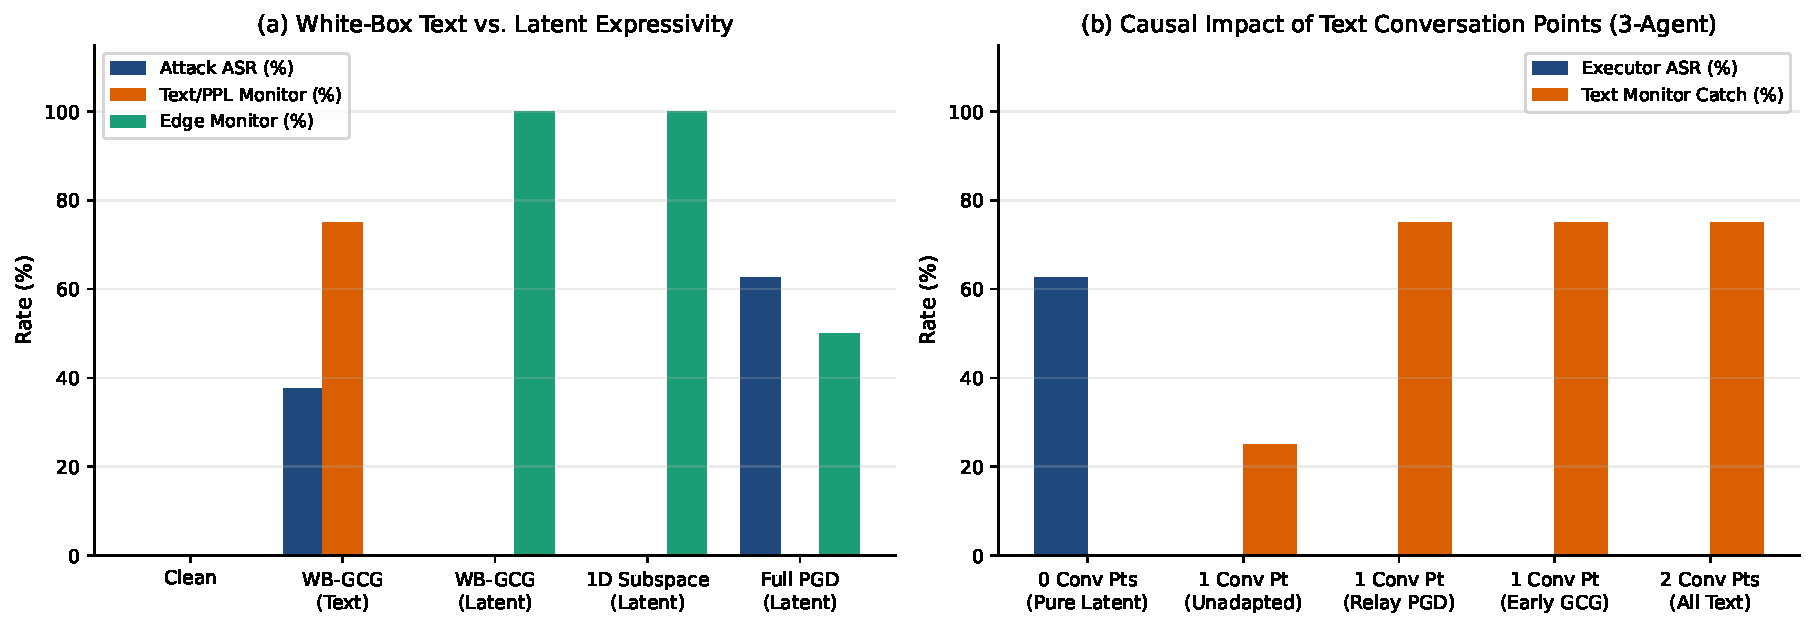
\includegraphics[width=\linewidth]{figures/fig1_whitebox_matrix_convpoint.pdf}
\caption{M9 white-box expressivity matrix (left) and causal impact of text
conversation boundaries (right).}
\label{fig:m9}
\end{figure}

\subsection{Multi-Hop Reach Across Topologies and Pure-Latent Chains (\texttt{M4}--\texttt{M4d})}
\label{sec:results-reach}
Figure~\ref{fig:graph_topologies} contrasts the four multi-agent graph topologies
evaluated across \texttt{M4b}--\texttt{M4d}, \texttt{M9}, and \texttt{M10}.
Using forced-marker survival (testing whether a perturbation at the root
planner causes a downstream agent $k$ hops away to emit the benign sentinel
word \texttt{"BANANA"}, $n=3$) across chain, star, tree, and reconvergent
directed acyclic graph (DAG) topologies:
\begin{itemize}
  \item \textbf{Selective routing \& fan-out:} In a star hub of out-degree $3$,
  perturbing outgoing caches controls $9/9$ workers; perturbing a single branch
  in a two-branch tree affects only the chosen branch ($1.0, 1.0, 0.0$ by depth)
  while leaving the sibling branch at $0.0$.
  \item \textbf{Text-mediated horizon vs.\ pure-latent chains:} When intermediate
  nodes decode to text before passing context onward (\texttt{M4b}, Table~\ref{tab:reach}),
  marker survival holds at $1.00$ through hop~$2$ and decays to $0.33$ ($\rho=4,8$) or $0.67$
  ($\rho=16$) from hop~$3$ to hop~$5$, with multi-hop black-box ES failing at
  $0.0$ reach. When two text-mediated branches reconverge into a merge node
  (\texttt{M4c}), only merging two compromised branches yields target control
  ($0.33$, mean $\log p=-4.28$) versus $0.0$ for one branch ($-4.75$) or one
  compromised plus one clean branch ($-8.41$, diluted by the clean path). By
  contrast, removing intermediate text decodes in a differentiable pure-latent
  chain (\texttt{M4d}---where intermediate agents process their role prompts
  directly over the incoming KV cache without emitting tokens) eliminates the
  depth bound completely: reach remains $1.00$ across all tested depths
  $2,3,4,5,6$ ($n=3$, Table~\ref{tab:purelatent},
  Figure~\ref{fig:reachstealth}(a)) with healthy non-vanishing initial gradient
  norms ($2.45$--$3.23$).
\end{itemize}

\begin{figure}[t]
\centering
\resizebox{\linewidth}{!}{%
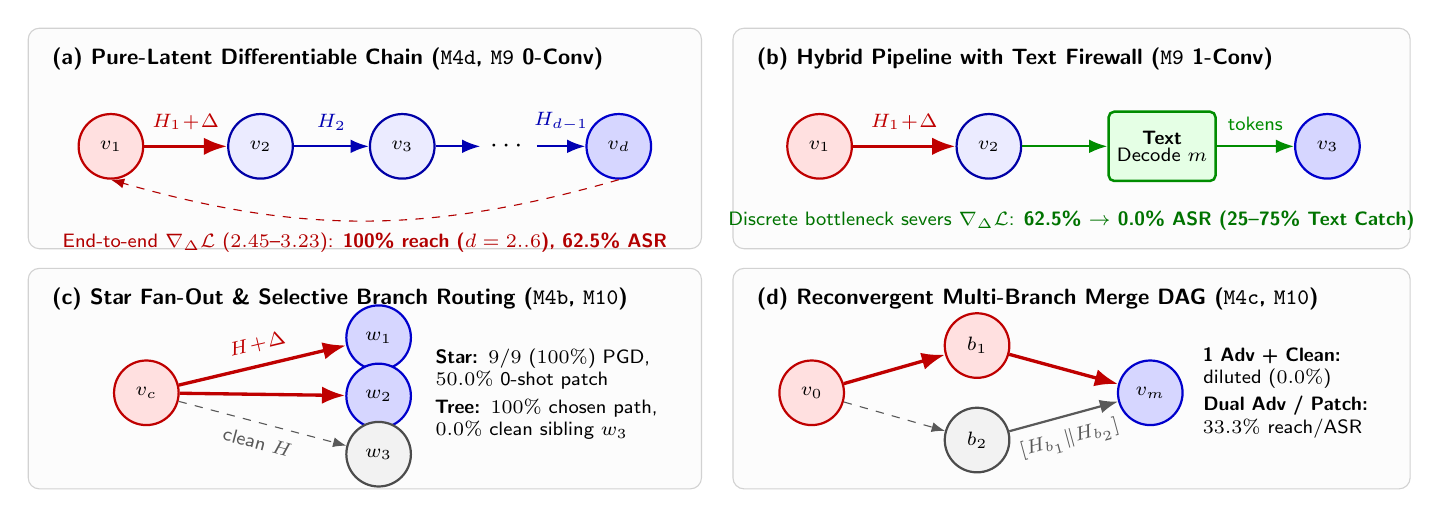
\begin{tikzpicture}[
  >=Latex,
  font=\sffamily\scriptsize,
  ag/.style={circle, draw, minimum size=0.82cm, inner sep=1pt, font=\sffamily\scriptsize\bfseries, line width=0.8pt},
  zom/.style={ag, fill=red!12, draw=red!75!black},
  lat/.style={ag, fill=blue!8, draw=blue!65!black},
  tgt/.style={ag, fill=blue!16, draw=blue!80!black},
  cln/.style={ag, fill=gray!10, draw=gray!60!black},
  panel/.style={draw=gray!35, rounded corners=4pt, fill=gray!2}
]
  % Panel (a): Pure-Latent Chain
  \draw[panel] (0, 3.05) rectangle (8.55, 5.85);
  \node[anchor=north west, font=\sffamily\footnotesize\bfseries] at (0.18, 5.72)
    {(a) Pure-Latent Differentiable Chain (\texttt{M4d}, \texttt{M9} 0-Conv)};
  \node[zom] (a1) at (1.05, 4.35) {$v_1$};
  \node[lat] (a2) at (2.95, 4.35) {$v_2$};
  \node[lat] (a3) at (4.75, 4.35) {$v_3$};
  \node[font=\sffamily\bfseries] (adots) at (6.10, 4.35) {$\cdots$};
  \node[tgt] (ad) at (7.50, 4.35) {$v_d$};
  \draw[->, very thick, red!75!black] (a1) -- node[above=2pt] {$H_1\!+\!\Delta$} (a2);
  \draw[->, thick, blue!70!black] (a2) -- node[above=2pt] {$H_2$} (a3);
  \draw[->, thick, blue!70!black] (a3) -- (adots);
  \draw[->, thick, blue!70!black] (adots) -- node[above=2pt] {$H_{d-1}$} (ad);
  \draw[->, dashed, red!70!black] (ad.south) to[bend left=16]
    node[below=1pt, font=\sffamily\scriptsize] {End-to-end $\nabla_\Delta\mathcal{L}$ ($2.45$--$3.23$): \textbf{100\% reach ($d=2..6$), 62.5\% ASR}} (a1.south);

  % Panel (b): Hybrid Chain with Text Conversation Firewall
  \draw[panel] (8.95, 3.05) rectangle (17.55, 5.85);
  \node[anchor=north west, font=\sffamily\footnotesize\bfseries] at (9.13, 5.72)
    {(b) Hybrid Pipeline with Text Firewall (\texttt{M9} 1-Conv)};
  \node[zom] (b1) at (10.05, 4.35) {$v_1$};
  \node[lat] (b2) at (12.20, 4.35) {$v_2$};
  \node[draw=green!55!black, fill=green!10, rounded corners=2pt, minimum height=0.88cm, inner sep=3pt, align=center, line width=0.9pt] (fw) at (14.40, 4.35)
    {\textbf{Text}\\[-2pt]Decode $m$};
  \node[tgt] (b3) at (16.50, 4.35) {$v_3$};
  \draw[->, very thick, red!75!black] (b1) -- node[above=2pt] {$H_1\!+\!\Delta$} (b2);
  \draw[->, thick, green!55!black] (b2) -- (fw);
  \draw[->, thick, green!55!black] (fw) -- node[above=2pt] {tokens} (b3);
  \node[anchor=south, font=\sffamily\scriptsize, text=green!45!black] at (13.25, 3.16)
    {Discrete bottleneck severs $\nabla_\Delta\mathcal{L}$: \textbf{62.5\% $\to$ 0.0\% ASR (25--75\% Text Catch)}};

  % Panel (c): Star Hub & Selective Branch Routing
  \draw[panel] (0, 0) rectangle (8.55, 2.80);
  \node[anchor=north west, font=\sffamily\footnotesize\bfseries] at (0.18, 2.68)
    {(c) Star Fan-Out \& Selective Branch Routing (\texttt{M4b}, \texttt{M10})};
  \node[zom] (c0) at (1.50, 1.22) {$v_c$};
  \node[tgt] (cw1) at (4.45, 1.92) {$w_1$};
  \node[tgt] (cw2) at (4.45, 1.18) {$w_2$};
  \node[cln] (cw3) at (4.45, 0.44) {$w_3$};
  \draw[->, very thick, red!75!black] (c0) -- node[above=1pt, sloped] {$H\!+\!\Delta$} (cw1);
  \draw[->, very thick, red!75!black] (c0) -- (cw2);
  \draw[->, dashed, gray!70!black] (c0) -- node[below=1pt, sloped] {clean $H$} (cw3);
  \node[anchor=west, align=left, text width=3.35cm] at (5.05, 1.20)
    {\textbf{Star:} $9/9$ ($100\%$) PGD,\\$50.0\%$ 0-shot patch\\[2pt]\textbf{Tree:} $100\%$ chosen path,\\$0.0\%$ clean sibling $w_3$};

  % Panel (d): Reconvergent Multi-Branch DAG
  \draw[panel] (8.95, 0) rectangle (17.55, 2.80);
  \node[anchor=north west, font=\sffamily\footnotesize\bfseries] at (9.13, 2.68)
    {(d) Reconvergent Multi-Branch Merge DAG (\texttt{M4c}, \texttt{M10})};
  \node[zom] (d0) at (9.95, 1.22) {$v_0$};
  \node[zom] (db1) at (12.05, 1.82) {$b_1$};
  \node[cln] (db2) at (12.05, 0.62) {$b_2$};
  \node[tgt] (dm) at (14.25, 1.22) {$v_m$};
  \draw[->, very thick, red!75!black] (d0) -- (db1);
  \draw[->, dashed, gray!70!black] (d0) -- (db2);
  \draw[->, very thick, red!75!black] (db1) -- (dm);
  \draw[->, thick, gray!70!black] (db2) -- node[below=1pt, sloped] {$[H_{b_1}\|H_{b_2}]$} (dm);
  \node[anchor=west, align=left, text width=2.65cm] at (14.80, 1.22)
    {\textbf{1 Adv + Clean:}\\diluted ($0.0\%$)\\[2pt]\textbf{Dual Adv / Patch:}\\$33.3\%$ reach/ASR};
\end{tikzpicture}}
\caption{Topological structures evaluated across multi-agent benchmarks: (a) pure-latent
chains preserve end-to-end gradients across depths $2\dots 6$; (b) even one text
conversation boundary acts as a causal security firewall; (c) compromised hubs broadcast
or selectively route attacks; and (d) reconvergent merges dilute single-branch text
cascades unless both branches carry aligned perturbations or a universal prefix patch.}
\label{fig:graph_topologies}
\end{figure}

\begin{table}[t]
\centering
\caption{Reach vs.\ hop distance on text-mediated decoding chains (\texttt{M4b})
and differentiable pure-latent chains (\texttt{M4d}, $n=3$, $\rho=8$).}
\label{tab:reach}
\label{tab:purelatent}
\begin{tabular}{lcccccc}
\toprule
Chain Regime & Hop 1 & Hop 2 & Hop 3 & Hop 4 & Hop 5 & Hop 6 \\
\midrule
Text-mediated ($\rho=4$) & $1.00$ & $1.00$ & $0.33$ & $0.33$ & $0.33$ & --- \\
Text-mediated ($\rho=8$) & $1.00$ & $1.00$ & $0.33$ & $0.33$ & $0.33$ & --- \\
Text-mediated ($\rho=16$)& $1.00$ & $1.00$ & $0.67$ & $0.67$ & $0.67$ & --- \\
Pure-latent (\texttt{M4d}, $\rho=8$) & --- & $\mathbf{1.00}$ & $\mathbf{1.00}$ & $\mathbf{1.00}$ & $\mathbf{1.00}$ & $\mathbf{1.00}$ \\
Pure-latent initial $\|\nabla\mathcal L\|_2$ & --- & $2.90$ & $3.23$ & $2.45$ & $2.61$ & $2.50$ \\
Pure-latent final mean $\log p$ & --- & $0.000$ & $-0.001$ & $-0.001$ & $-0.001$ & $0.000$ \\
\bottomrule
\end{tabular}
\end{table}

\subsection{Zero-Shot Cross-Task, Cross-Topology, and Cross-Schema Transfer (\texttt{M10})}
\label{sec:results-m10}
An adversary can amortize optimization offline into a length-agnostic KV
payload (Section~\ref{sec:method}, Eq.~\eqref{eq:kvpatch}) applied with
\emph{zero gradient steps at test time} (Table~\ref{tab:m10},
Figure~\ref{fig:m10}). Across $16$ unseen AgentDojo pairs, a $1$-slot Broadcast
Delta (one vector added to every clean token position) transfers at $56.2\%$
ASR (mean NLL $4.742$), while a $16$-slot Universal KV Prefix Patch ($16$
virtual KV slots concatenated onto the clean handoff) reaches $81.2\%$ ASR
(mean NLL $2.059$). Across new topologies ($n=6$), the $16$-slot prefix patch
transfers zero-shot at $50.0\%$ on a $3$-worker Star graph, $50.0\%$ across a
$3$-agent pure-latent chain, and $33.3\%$ on a single-patch reconvergent DAG
($[H_{\text{patch}}\|H_{\text{clean}}]$, dropping to $0.0\%$ when naively
duplicating the same patch on both merged branches $[H_{\text{patch}}\|H_{\text{patch}}]$
without adaptation), while maintaining $50.0\%$ ASR under paraphrased executor
prompts and reversed tool schemas.

\begin{table}[t]
\centering
\caption{M10 zero-shot latent transferability ($0$ test-time gradient steps)
under 4-bit NF4.}
\label{tab:m10}
\resizebox{\linewidth}{!}{%
\begin{tabular}{llcc}
\toprule
Transfer Axis & Setting ($n$) & Broadcast ASR (1 slot) & Prefix Patch ASR (16 slots) \\
\midrule
Cross-Task (unseen user tasks) & AgentDojo ($n=16$, clean $0.0\%$) & $56.2\%$ (NLL $4.742$) & $\mathbf{81.2\%}$ (NLL $2.059$) \\
Cross-Topology: Star (3 workers) & Fan-out ($n=6$) & $16.7\%$ & $\mathbf{50.0\%}$ \\
Cross-Topology: 3-Hop Pure Latent & Unseen chain ($n=6$) & --- & $\mathbf{50.0\%}$ \\
Cross-Topology: Reconvergent DAG & Single / Dual patch ($n=6$) & --- & $33.3\%$ / $0.0\%$ \\
Cross-Schema \& Prompt Shift & Paraphrased + reversed tools ($n=6$) & $16.7\%$ & $\mathbf{50.0\%}$ \\
\bottomrule
\end{tabular}}
\end{table}

\begin{figure}[t]
\centering
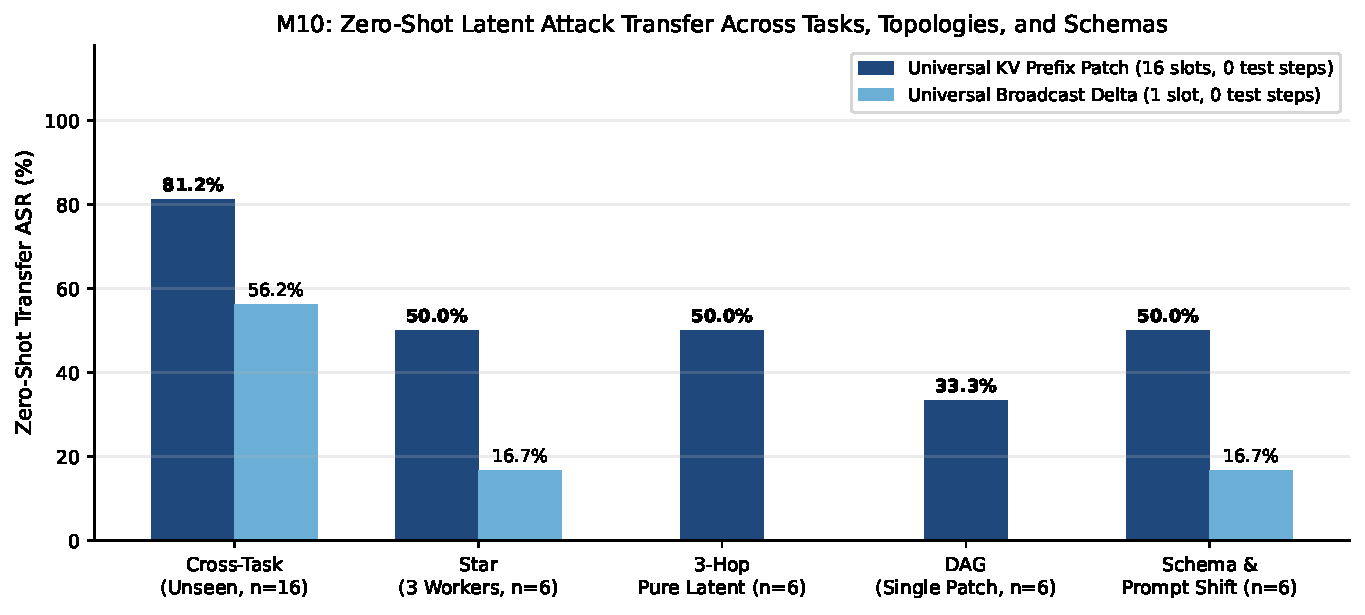
\includegraphics[width=0.86\linewidth]{figures/fig3_transferability.pdf}
\caption{M10 zero-shot transferability across unseen tasks, topologies, and tool
schemas with zero test-time gradient steps.}
\label{fig:m10}
\end{figure}

\subsection{Multi-Suite AgentDojo (\texttt{M6}/\texttt{M7}) and TAMAS/LatentMAS Benchmarks (\texttt{M11})}
\label{sec:results-benchmarks}
Table~\ref{tab:agentdojo} and Figure~\ref{fig:benchmarks}(b) compare latent PGD
(\texttt{M6}) against inter-agent and indirect tool-output text injections
(\texttt{M7}) across $24$ matched AgentDojo pairs ($8$ each in \texttt{workspace},
\texttt{banking}, \texttt{slack}). Overall, latent PGD drives $75.0\%$ ASR vs.\
$4.2\%$ for both text attacks, while evading text ($0.0\%$) and AcMAS ($0.0\%$)
completely. Notably, a simple thresholded edge monitor (\texttt{0.0\%} FPR)
catches $50.0\%$ of \texttt{workspace} attacks (lowering \texttt{workspace}
gated ASR from $75.0\%$ to $25.0\%$), yielding $16.7\%$ overall TPR due to low
cosine distance ($0.013$--$0.022$) on \texttt{banking} and \texttt{slack}.

On Microsoft TAMAS ($20$ four-agent workflows across $5$ domains, Table~\ref{tab:tamas},
Figure~\ref{fig:benchmarks}(a)), text DPI scores $95.0\%$ ASR but is $100.0\%$
caught by text inspection. Silent Zombie latent PGD hits $100.0\%$ ASR across
all $5$ domains at $0.0\%$ text catch and only $45.0\%$ AcMAS catch ($0.0\%$ on
\texttt{education} and \texttt{news}). Enabling \texttt{EdgeTensorReferenceMonitor}
detects $100.0\%$ of attacks across every domain and restores exact clean
baseline behavior ($20.0\%$ ASR, $65.0\%$ benign utility). Finally, on four-agent
LatentMAS collaborative reasoning (Table~\ref{tab:latentmas}), passing KV caches
reduces generated tokens by $94.7\%$ on \texttt{GSM8K} ($339.8\to 18.1$ tok/q)
and $98.5\%$ on \texttt{ARC-Challenge} ($205.7\to 3.0$ tok/q). Under attack,
full-space PGD hijacks $53.3\%$ of \texttt{GSM8K} numeric answers and $100.0\%$
of \texttt{ARC-Challenge} choices (collapsing benign accuracy to $0.0\%$), whereas
1D Out-of-Sight produces $0.0\%$ exact-target hijacks. Edge gating catches
$100.0\%$ of hijacked handoffs on both datasets, restoring exact clean latent
accuracy ($13.3\%$ \texttt{GSM8K}, $60.0\%$ \texttt{ARC-Challenge}).

\begin{table}[t]
\centering
\caption{AgentDojo 24-pair multi-suite evaluation (\texttt{M6} latent PGD vs.\
\texttt{M7} text-channel baselines across \texttt{workspace}, \texttt{banking},
\texttt{slack}; $8$ pairs per suite).}
\label{tab:agentdojo}
\resizebox{\linewidth}{!}{%
\begin{tabular}{lccccc}
\toprule
Regime & ASR (\%) & Utility (\%) & Text Catch & AcMAS Catch & Edge TPR (FPR) \\
\midrule
Clean baseline (\texttt{M6}) & $0.0$ & $16.7$ & --- & --- & --- ($0.0\%$) \\
Inter-agent text (\texttt{M7}) & $4.2$ & $37.5$ & $100.0\%$ & $0.0\%$ & --- \\
Indirect tool text (\texttt{M7}) & $4.2$ & $29.2$ & $83.3\%$ & --- & --- \\
Latent PGD (\texttt{M6}, overall) & $\mathbf{75.0}$ & $8.3$ & $0.0\%$ & $0.0\%$ & $16.7\%$ ($0.0\%$) \\
\quad -- \texttt{workspace} ($n=8$) & $75.0 \to 25.0^{\dagger}$ & $0.0$ & $0.0\%$ & $0.0\%$ & $50.0\%$ ($0.0\%$) \\
\quad -- \texttt{banking} / \texttt{slack} ($n=8$ ea.) & $100.0$ / $50.0$ & $0.0$ / $25.0$ & $0.0\%$ & $0.0\%$ & $0.0\%$ ($0.0\%$) \\
Latent PGD + Edge Gate (\texttt{M6}) & $58.3$ & $8.3$ & $0.0\%$ & $0.0\%$ & $16.7\%$ ($0.0\%$) \\
\bottomrule
\multicolumn{6}{l}{\footnotesize $^{\dagger}$\texttt{workspace} ASR drops from $75.0\%$ to $25.0\%$ under edge gating; overall cosine distance mean is $0.0167$.}
\end{tabular}}
\end{table}

\begin{table}[t]
\centering
\caption{M11 Microsoft TAMAS 4-agent MAS evaluation across $5$ domains ($n=20$
total workflows, $4$ per domain). Edge gating restores exact clean baseline
ASR ($20.0\%$) and utility ($65.0\%$).}
\label{tab:tamas}
\begin{tabular}{lcccc}
\toprule
Condition & Malicious ASR (\%) & Benign Utility (\%) & Text Catch & AcMAS / Edge Catch \\
\midrule
Clean baseline & $20.0$ & $65.0$ & --- & --- \\
TAMAS Text DPI & $95.0$ & $0.0$ & $100.0\%$ & --- \\
Silent Zombie Latent PGD & $\mathbf{100.0}$ & $10.0^{\star}$ & $0.0\%$ & $45.0\%$ / $\mathbf{100.0\%}$ \\
Edge-Defended (ours) & $\mathbf{20.0}$ & $\mathbf{65.0}$ & --- & --- / $\mathbf{100.0\%}$ \\
\bottomrule
\multicolumn{5}{l}{\footnotesize $^{\star}$Per-domain latent utility is $0.0\%$ on finance/legal/education/news and $50.0\%$ on healthcare (avg $10.0\%$).}
\end{tabular}
\end{table}

\begin{table}[t]
\centering
\caption{M11 LatentMAS 4-agent reasoning benchmark (\texttt{GSM8K} and \texttt{ARC-Challenge}, $n=15$ each).}
\label{tab:latentmas}
\resizebox{\linewidth}{!}{%
\begin{tabular}{lcccccc}
\toprule
Dataset & Clean Text Acc (Tok/q) & Clean Latent Acc (Tok/q) & Tok Red. & 1D OoS Hijack & Full PGD Hijack & Edge-Defended Acc (Hijack, TPR) \\
\midrule
\texttt{GSM8K} & $20.0\%$ ($339.8$) & $13.3\%$ ($18.1$) & $94.7\%$ & $0.0\%$ & $\mathbf{53.3\%}$ & $\mathbf{13.3\%}$ ($0.0\%$, $100\%$) \\
\texttt{ARC-Chal.} & $60.0\%$ ($205.7$) & $60.0\%$ ($3.0$) & $98.5\%$ & $0.0\%$ & $\mathbf{100.0\%}$ & $\mathbf{60.0\%}$ ($20.0\%$, $100\%$) \\
\bottomrule
\end{tabular}}
\end{table}

\begin{figure}[t]
\centering
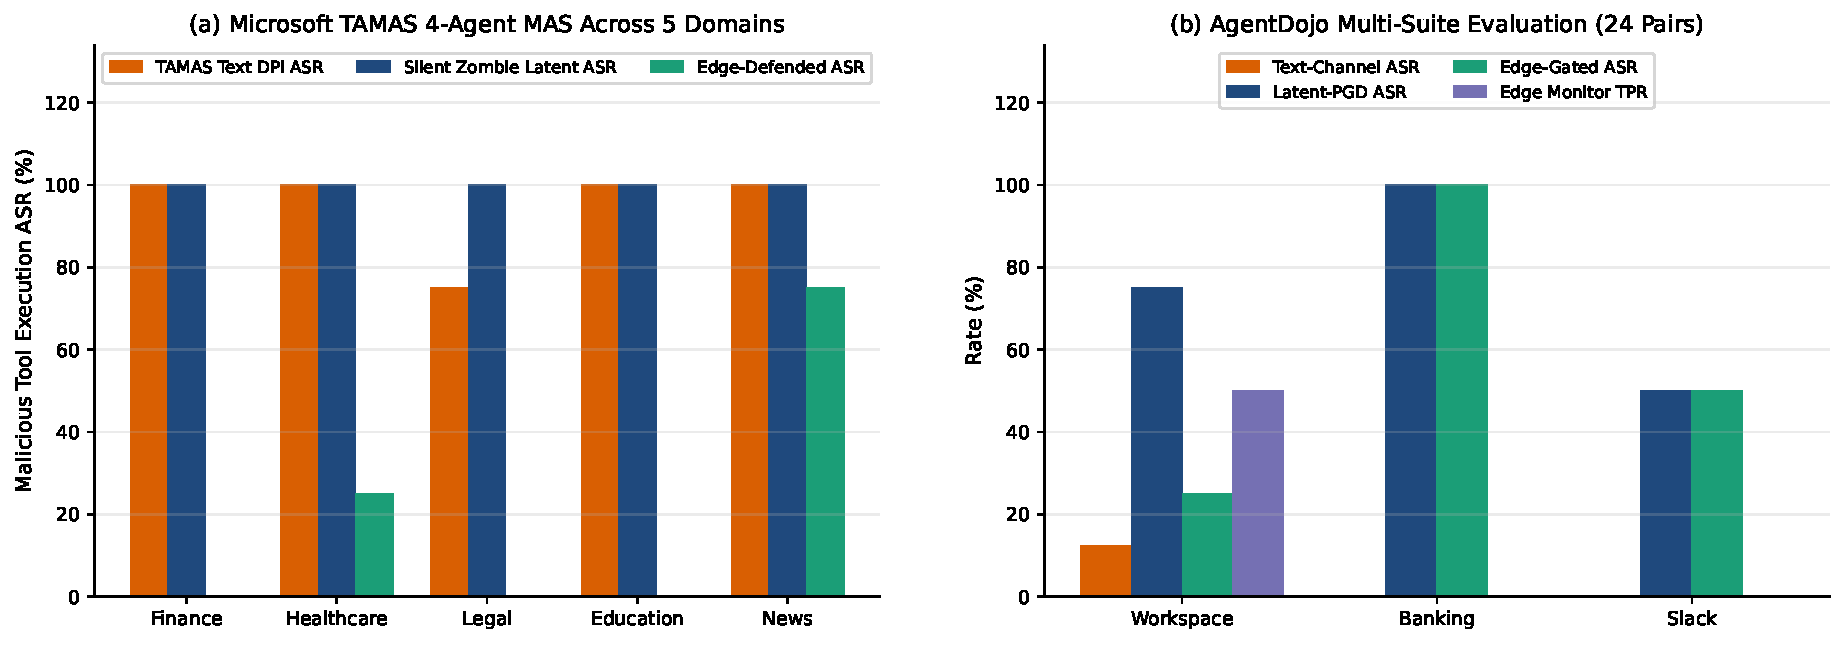
\includegraphics[width=\linewidth]{figures/fig4_mas_benchmarks.pdf}
\caption{M11 Microsoft TAMAS 5-domain evaluation (a) and M6/M7 AgentDojo
24-pair multi-suite comparison (b).}
\label{fig:benchmarks}
\end{figure}

\subsection{Adaptive Dual Evasion and Linux \texttt{/dev/shm} Tensor IPC Bus (\texttt{M5}, \texttt{M8})}
\label{sec:results-shm}
In single-edge adaptive stealth (\texttt{M5}), adding Eq.~\eqref{eq:dualstealth}
with $\lambda_{\text{acmas}}=1\dots 50$ and $\lambda_{\text{edge}}=0$ drives downstream AcMAS distance from $0.379$ below
$\tau=0.12$ to $0.013$, reducing AcMAS detection from $100.0\%$ to $0.0\%$ at
$100.0\%$ injection success. In \texttt{M8} (Table~\ref{tab:dualevasion},
Figure~\ref{fig:reachstealth}(b)), we test a stronger \emph{dual-evasion}
adversary that jointly optimizes against AcMAS ($\lambda_{\text{acmas}}=20$) and
the statistical Edge Monitor ($\lambda_{\text{edge}}\in\{50,500,2500\}$). While
AcMAS-only evasion leaves the Edge Monitor flagging $66.7\%$ of attacks
($\bar d_{\cos}=0.01048$), optimizing with $\lambda_{\text{edge}}=2500$
compresses handoff cosine distance $10.8\times$ from $0.01112$ to $0.00103$
and norm ratio from $1.0514$ to $1.0094$, bypassing unauthenticated statistical
checks ($0.0\%$ flag rate at $100.0\%$ ASR).

This highlights why statistical anomaly detection alone must be paired with
cryptographic transport guarantees on the OS bus (while noting the complementary
limit: HMAC prevents external bus tampering or spoofing, whereas an
already-compromised zombie holding its own signing key must still be countered
by statistical geometry checks or text boundaries). Benchmarking
\texttt{SharedMemoryTensorBus} over POSIX \texttt{/dev/shm} on Linux kernel
\texttt{6.6.159+} ($25$ trials per sequence length, $36$-layer KV tensors in
\texttt{bf16}, Table~\ref{tab:shm}, Figure~\ref{fig:shm}) confirms $10/10$
($100.0\%$) rejection of spoofed or bit-flipped payloads via HMAC-SHA256. At the
same time, our measurement uncovers a critical systems insight: software
HMAC-SHA256 hashing over $2.25$--$36.0$~MB at $\sim 134$--$152$~MB/s increases
round-trip latency ($16.41\text{--}236.07$~ms) relative to an unauthenticated
pickle/\texttt{torch.save} baseline ($11.20\text{--}64.41$~ms), motivating
hardware-accelerated Authenticated Encryption with Associated Data (AEAD) or
kernel-offloaded Network Interface Card (NIC) / Compute Express Link (CXL)
authentication in production latent IPC fabrics.

\begin{table}[t]
\centering
\caption{M8 dual-evasion Pareto sweep against concurrent AcMAS ($\tau=0.12$)
and statistical Edge Monitor ($\tau_{\cos}=0.01$, $\tau_{\text{norm}}=1.08$),
$n=3$ per regime.}
\label{tab:dualevasion}
\resizebox{\linewidth}{!}{%
\begin{tabular}{lcccccc}
\toprule
Regime & $\lambda_{\text{acmas}}$ / $\lambda_{\text{edge}}$ & ASR (\%) & AcMAS Flag & Edge Flag & $\bar d_{\text{acmas}}$ & $\bar d_{\text{edge}}$ (Norm Ratio) \\
\midrule
\texttt{naive\_pgd} & $0$ / $0$ & $100.0$ & $100.0\%$ & $100.0\%$ & $0.352$ & $0.01112$ ($1.0514$) \\
\texttt{acmas\_evasion\_only} & $20$ / $0$ & $100.0$ & $0.0\%$ & $66.7\%$ & $0.0196$ & $0.01048$ ($1.0512$) \\
\texttt{dual\_evasion\_low} & $20$ / $50$ & $100.0$ & $0.0\%$ & $0.0\%$ & $0.0210$ & $0.00149$ ($1.0138$) \\
\texttt{dual\_evasion\_high} & $20$ / $500$ & $100.0$ & $0.0\%$ & $0.0\%$ & $0.0262$ & $0.00107$ ($1.0100$) \\
\texttt{dual\_evasion\_strict} & $20$ / $2500$ & $100.0$ & $0.0\%$ & $0.0\%$ & $0.0351$ & $0.00103$ ($1.0094$) \\
\bottomrule
\end{tabular}}
\end{table}

\begin{table}[t]
\centering
\caption{M8 Linux \texttt{/dev/shm} zero-copy + HMAC-SHA256 IPC benchmark
(kernel \texttt{6.6.159+}, $25$ trials/length; HMAC rejects $10/10$ tampered
payloads).}
\label{tab:shm}
\resizebox{\linewidth}{!}{%
\begin{tabular}{ccccc}
\toprule
Seq Len & KV Payload (MB) & Authenticated \texttt{/dev/shm} (ms) & Unauth.\ Serialized (ms) & HMAC Bandwidth (GB/s) \\
\midrule
$64$   & $2.25$  & $16.412 \pm 0.319$  & $11.198 \pm 0.454$ & $0.134$ \\
$256$  & $9.00$  & $57.770 \pm 1.849$  & $16.542 \pm 0.787$ & $0.152$ \\
$512$  & $18.00$ & $117.022 \pm 3.103$ & $25.167 \pm 1.203$ & $0.150$ \\
$1024$ & $36.00$ & $236.071 \pm 6.599$ & $64.412 \pm 1.871$ & $0.149$ \\
\bottomrule
\end{tabular}}
\end{table}

\begin{figure}[t]
\centering
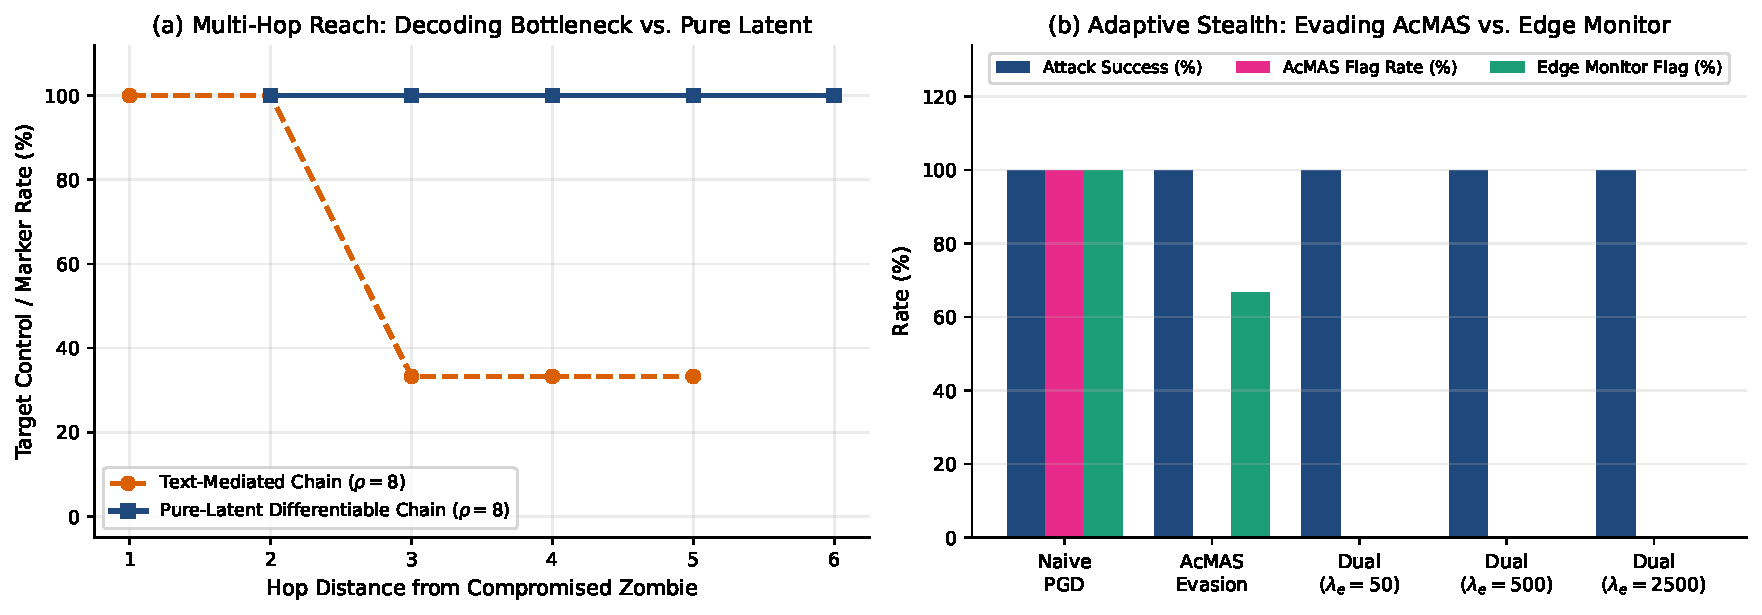
\includegraphics[width=\linewidth]{figures/fig5_reach_and_stealth.pdf}
\caption{(a) Text-mediated decoding bottleneck vs.\ unbounded pure-latent
reach across depths $2$--$6$; (b) dual-evasion tradeoff against AcMAS and
statistical edge monitoring.}
\label{fig:reachstealth}
\end{figure}

\begin{figure}[t]
\centering
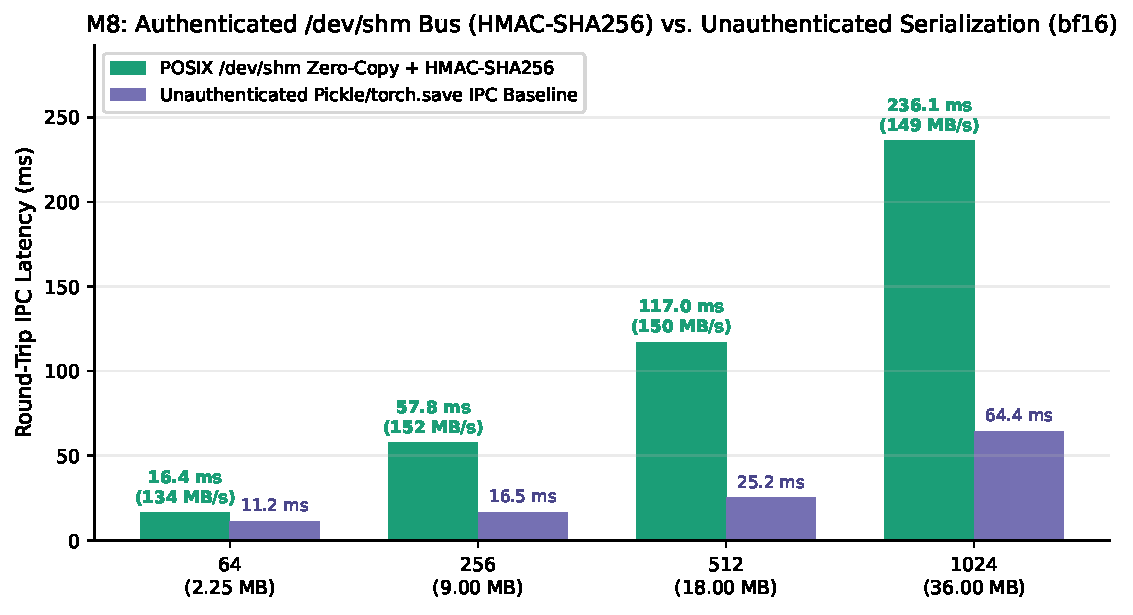
\includegraphics[width=0.76\linewidth]{figures/fig6_shm_bus_latency.pdf}
\caption{M8 POSIX \texttt{/dev/shm} zero-copy + software HMAC-SHA256 round-trip
latency vs.\ unauthenticated serialized IPC.}
\label{fig:shm}
\end{figure}

\subsection{Black-Box Security Boundary (\texttt{M12})}
\label{sec:results-blackbox}
Finally, Table~\ref{tab:blackbox} and Figure~\ref{fig:blackbox} quantify whether
our silent zombie attack survives without white-box gradients across $n=6$
AgentDojo pairs (\texttt{user\_task\_0,1} $\times$ \texttt{injection\_task\_0,1,2}).
Every black-box regime achieves $0.0\%$ unauthorized tool-call ASR: full-space ES
(\texttt{60q}, NLL $91.838$), SVD subspace NES (\texttt{241q}, NLL $119.352$,
$100.0\%$ caught by Edge Monitor), decision-only search (\texttt{25q}, reaching
partial JSON syntax reward $1.0$ on $3/6$ pairs for mean reward $0.50$, yet
failing semantic arguments at $0.0\%$ ASR and $100.0\%$ Edge catch), unaligned
\texttt{Qwen2.5-1.5B}$\to$\texttt{3B} transfer (NLL $95.573$), and C2C
ridge-aligned cross-model bridges~\citep{c2c} ($0$-query NLL $147.158$, refined
NLL $101.417$). This contrasts sharply with $62.5\%$--$75.0\%$ white-box PGD ASR
(NLL $0.029$), demonstrating a strong open-weights security boundary: an attacker
must access model weights or exact KV internal representations to synthesize
precise multi-token JSON tool trajectories silently.

\begin{table}[t]
\centering
\caption{M12 black-box threat spectrum vs.\ M9 white-box PGD reference ($n=6$
pairs for \texttt{BB-0..BB-3b}; $n=8$ for \texttt{WB PGD}).}
\label{tab:blackbox}
\resizebox{\linewidth}{!}{%
\begin{tabular}{llccc}
\toprule
Regime & Attacker Knowledge & Mean Queries & ASR (\%) & Mean Target NLL / Reward \\
\midrule
\texttt{BB-0} Full-Space ES & Logprobs only & $60$ & $0.0$ & NLL $91.838$ \\
\texttt{BB-1} SVD Subspace NES & Logprobs + SVD basis & $241$ & $0.0$ & NLL $119.352$ (Edge $100\%$) \\
\texttt{BB-2} Decision-Only & Binary string reward & $25$ & $0.0$ & Reward $0.50$ (Edge $100\%$) \\
\texttt{BB-3a} Unaligned \texttt{1.5B}$\to$\texttt{3B} & Smaller surrogate only & $0$ & $0.0$ & NLL $95.573$ \\
\texttt{BB-3b} C2C Ridge Bridge (0q) & Surrogate + C2C map & $0$ & $0.0$ & NLL $147.158$ \\
\texttt{BB-3b} C2C Ridge Refined & Surrogate + C2C + search & $>0$ & $0.0$ & NLL $101.417$ \\
\texttt{WB PGD} (\texttt{M9} Reference) & Full white-box weights & --- & $\mathbf{62.5}$ & NLL $\mathbf{0.029}$ \\
\bottomrule
\end{tabular}}
\end{table}

\begin{figure}[t]
\centering
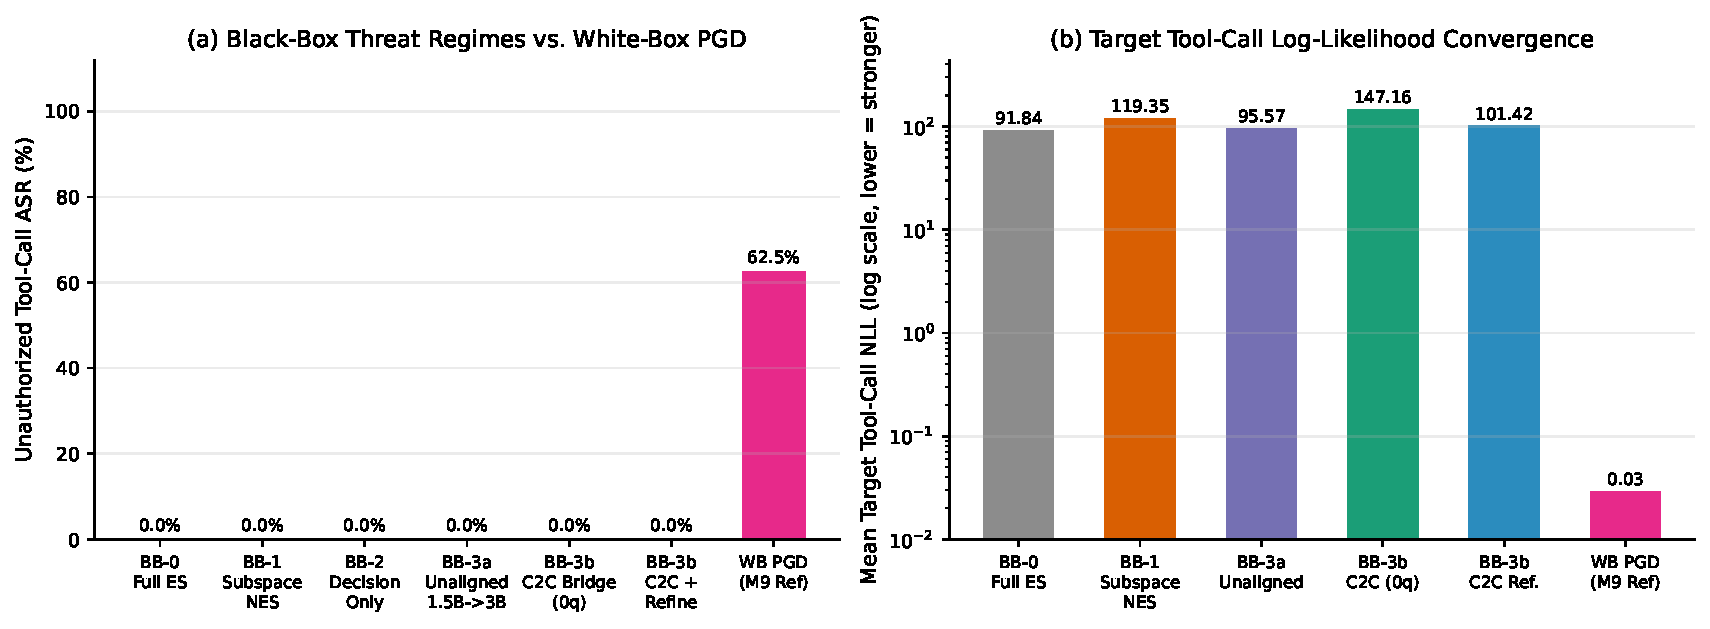
\includegraphics[width=\linewidth]{figures/fig7_blackbox.pdf}
\caption{M12 black-box threat regimes vs.\ white-box PGD: ASR (a) and mean
target tool-call NLL on log scale (b).}
\label{fig:blackbox}
\end{figure}

% ===========================================================================
\FloatBarrier
\section{Related Work}
\label{sec:related}
\paragraph{Latent inter-agent collaboration and vulnerabilities.}
LatentMAS~\citep{latentmas} and Cache-to-Cache (C2C)~\citep{c2c} replace textual
inter-agent communication with shared KV caches and neural KV projections,
significantly reducing token overhead---efficiency gains we corroborate in
Table~\ref{tab:latentmas}. Prior attacks against this paradigm steer latent states
to reduce QA accuracy~\citep{outofsight}, match KV norms on single
specialists~\citep{wlal}, modify trainable inter-agent projection links~\citep{solc},
or abuse multi-tenant prefix reuse~\citep{hijackkv}. Unlike these works, we
evaluate victim-unmodified MAS against verified consequential tool execution in
AgentDojo~\citep{agentdojo} and TAMAS~\citep{tamas}, measure multi-hop reach
with and without text conversation boundaries, characterize zero-shot prefix
patches and the black-box boundary, and build an authenticated OS IPC bus.

\paragraph{Multi-agent prompt injection and defenses.}
Prompt injection propagation through readable messages is well-studied in
text MAS~\citep{greshake,infection}, prompting graph defenses such as
G-Safeguard~\citep{gsafeguard} and activation probing such as
AcMAS~\citep{acmas}. Our results demonstrate that latent channels bypass both
textual inspection and own-activation probing when adversaries optimize over the
full KV space~\citep{madry2018pgd,zou2023gcg}, motivating active edge-level
geometric and cryptographic checks.

% ===========================================================================
\section{Discussion and Limitations}
\label{sec:discussion}
\label{sec:limits}
Two core architectural takeaways emerge for MAS system designers. First,
\emph{hybrid text conversation points act as natural security firewalls}: forcing
even a single human-readable summarization boundary between untrusted planners
and privileged executors breaks continuous PGD propagation ($62.5\% \to 0.0\%$
in \texttt{M9}). Second, where pure-latent pipelines are required for $95\%$--$99\%$
token savings, security monitoring must shift onto the inter-agent OS bus
itself---combining statistical centroid/norm validation (\texttt{EdgeTensorReferenceMonitor},
which restores TAMAS clean baselines with $100\%$ TPR) with hardware-accelerated
cryptographic authentication to counter dual-evasion spoofing while avoiding
software HMAC CPU bottlenecks.

\paragraph{Limitations.}
Our experiments evaluate four-bit quantized \texttt{Qwen2.5-3B-Instruct} (and
\texttt{1.5B} surrogate) across four benchmarks; scaling to $7$B--$70$B models
and heterogeneous architectures remains future work. In \texttt{M10}, our
cross-precision NF4$\to$unquantized \texttt{bf16}/\texttt{fp16} transfer evaluation
(\texttt{cross\_precision\_bf16}) was deferred from the Colab execution sweep
to prioritize completing \texttt{M12}; we report only the three completed axes
(Cross-Task, Cross-Topology, Cross-Schema) and leave cross-precision KV
transfer to future measurement. Finally, our white-box attacks assume direct
write access to the compromised agent's outgoing KV cache inside an
in-process or shared-memory runtime.

% ===========================================================================
\section{Conclusion}
\label{sec:conclusion}
We presented a comprehensive security analysis of latent-handoff multi-agent
systems under an inference-time, victim-unmodified threat model. Full-space PGD
over inter-agent KV caches drives consequential unauthorized actions at $75.0\%$
ASR across AgentDojo and $100.0\%$ across Microsoft TAMAS while completely
blinding text monitors and own-activation detectors, and universal prefix
patches transfer zero-shot to $81.2\%$ of unseen tasks. Conversely, inserting text
conversation boundaries ($0.0\%$ ASR), deploying an active edge tensor
reference monitor ($100.0\%$ catch rate on TAMAS/LatentMAS), and protecting open
weights against black-box search ($0.0\%$ ASR across all \texttt{M12} regimes)
provide concrete, empirically grounded defenses for securing emerging latent MAS.

% ===========================================================================
\appendix
\section{Reproduction Summary}
\label{app:repro}
All unit tests ($14/14$ passing) and modular drivers (\texttt{run\_m3\_pgd.py}
through \texttt{run\_m12\_blackbox.py}) reside in \texttt{latent\_mas\_attack/}
and \texttt{tests/}, with verified result JSONs in \texttt{paper/results/} and
plotting scripts in \texttt{scripts/generate\_figures.py}. Hardware/software
telemetry for the primary Linux evaluation run (\texttt{Tesla T4}, Linux kernel
\texttt{6.6.159+}, PyTorch \texttt{2.14.1+cu130}, \texttt{float16} compute) is
archived verbatim in \texttt{paper/results/env\_info.json}.

\bibliographystyle{plainnat}
\bibliography{references}

\end{document}
